\documentclass[11pt]{article}
\usepackage[margin=1in]{geometry}
\usepackage{booktabs}
\usepackage{graphicx}
\usepackage{siunitx}
\usepackage{caption}

\sisetup{
  detect-weight=true,
  separate-uncertainty=true,
  table-number-alignment=center,
}

\title{PnP Inversion Results: Paper Reference and SD1.5 LoRA Evaluation}
\date{}

\begin{document}
\maketitle

\section{PnP Inversion Paper Results}

Figure~\ref{fig:paper-results} reproduces the uploaded PnP inversion results from
the paper verbatim.

\begin{figure}[htbp]
  \centering
  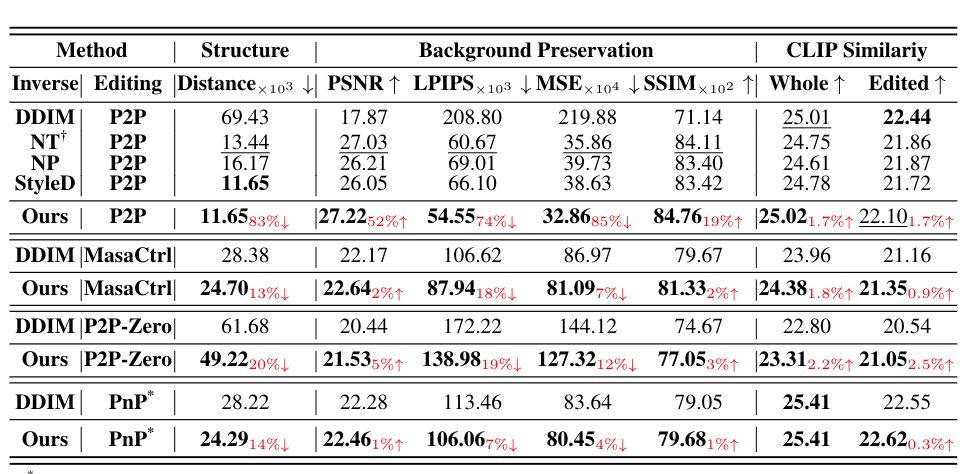
\includegraphics[width=\linewidth]{pnp_inversion_results.png}
  \caption{Uploaded PnP inversion results from the paper.}
  \label{fig:paper-results}
\end{figure}

\clearpage
\section{SD1.5 LoRA Editing Results}

Table~\ref{tab:lora-pnp} reports mean $\pm$ population standard deviation over
the generated PIE-Bench results. Structure distance and LPIPS are scaled by $10^3$, MSE by $10^4$, and SSIM by $10^2$. Structure distance, LPIPS, and MSE are lower-is-better.
PSNR, SSIM, and CLIP scores are higher-is-better. The unedited-region metrics have
$n=556$ valid images because 144 PIE-Bench samples have no unedited region; all other
metrics use $n=700$.

\begin{table*}[htbp]
  \centering
  \small
  \caption{SD1.5 LoRA inversion on PIE-Bench with four editing methods.}
  \label{tab:lora-pnp}
  \resizebox{\textwidth}{!}{%
  \begin{tabular}{llrrrrrrrr}
    \toprule
    Editor & Rank & $\alpha$ & Structure ($\times 10^3$) $\downarrow$ & PSNR (dB) $\uparrow$ & LPIPS ($\times 10^3$) $\downarrow$ &
    MSE ($\times 10^4$) $\downarrow$ & SSIM ($\times 10^2$) $\uparrow$ & CLIP target $\uparrow$ & CLIP target (edit) $\uparrow$ \\
    \midrule
    PnP & r8  & 4  & $27.347 \pm 25.199$ & $22.2856 \pm 4.4530$ & $114.421 \pm 64.992$ & $83.254 \pm 60.374$ & $79.430 \pm 12.895$ & $25.6356 \pm 3.7154$ & $22.7179 \pm 4.7900$ \\
    PnP & r16 & 8  & $27.178 \pm 24.677$ & $22.3235 \pm 4.5144$ & $114.157 \pm 64.640$ & $82.440 \pm 59.256$ & $79.455 \pm 12.868$ & $25.6510 \pm 3.7378$ & $22.7767 \pm 4.8115$ \\
    PnP & r32 & 16 & $27.077 \pm 24.675$ & $22.3287 \pm 4.2773$ & $113.467 \pm 64.744$ & $81.698 \pm 58.700$ & $79.540 \pm 12.846$ & $25.6141 \pm 3.7604$ & $22.8051 \pm 4.8448$ \\
    \midrule
    P2P & r8  & 4  & $70.454 \pm 39.602$ & $17.8081 \pm 3.9172$ & $211.100 \pm 106.517$ & $221.318 \pm 145.762$ & $71.370 \pm 15.855$ & $25.3785 \pm 3.6391$ & $22.5749 \pm 4.5293$ \\
    P2P & r16 & 8  & $70.401 \pm 38.766$ & $17.8174 \pm 3.9122$ & $210.983 \pm 106.113$ & $220.656 \pm 144.994$ & $71.366 \pm 15.785$ & $25.3632 \pm 3.6187$ & $22.5695 \pm 4.5753$ \\
    P2P & r32 & 16 & $70.469 \pm 40.181$ & $17.8209 \pm 3.8950$ & $210.948 \pm 106.102$ & $220.220 \pm 145.218$ & $71.394 \pm 15.868$ & $25.3638 \pm 3.5874$ & $22.5507 \pm 4.5221$ \\
    \midrule
    MasaCtrl & r8  & 4  & $26.557 \pm 19.334$ & $22.2538 \pm 4.6902$ & $106.534 \pm 61.469$ & $87.907 \pm 70.679$ & $80.285 \pm 12.743$ & $24.1593 \pm 3.8027$ & $21.1248 \pm 4.6742$ \\
    MasaCtrl & r16 & 8  & $26.489 \pm 19.745$ & $22.2899 \pm 4.7143$ & $105.299 \pm 60.893$ & $87.572 \pm 72.821$ & $80.369 \pm 12.767$ & $24.2166 \pm 3.8033$ & $21.1784 \pm 4.6505$ \\
    MasaCtrl & r32 & 16 & $26.667 \pm 19.936$ & $22.2832 \pm 4.6892$ & $105.378 \pm 61.602$ & $87.273 \pm 72.328$ & $80.452 \pm 12.654$ & $24.1279 \pm 3.7872$ & $21.1821 \pm 4.6847$ \\
    \midrule
    Pix2Pix-Zero & r8  & 4  & $51.593 \pm 51.822$ & $21.3347 \pm 5.5786$ & $145.870 \pm 119.774$ & $140.594 \pm 169.229$ & $76.981 \pm 15.830$ & $23.4618 \pm 4.2800$ & $20.9859 \pm 4.6982$ \\
    Pix2Pix-Zero & r16 & 8  & $52.385 \pm 53.039$ & $21.2614 \pm 5.5527$ & $146.894 \pm 119.914$ & $142.566 \pm 177.526$ & $76.899 \pm 15.841$ & $23.3541 \pm 4.3416$ & $21.0480 \pm 4.7030$ \\
    Pix2Pix-Zero & r32 & 16 & $51.652 \pm 52.878$ & $21.2867 \pm 5.5543$ & $147.021 \pm 120.497$ & $140.933 \pm 170.816$ & $77.032 \pm 15.819$ & $23.4061 \pm 4.4355$ & $21.0405 \pm 4.7464$ \\
    \bottomrule
  \end{tabular}
  }
\end{table*}

\begin{table}[htbp]
  \centering
  \small
  \caption{CLIP similarity to the source prompt. This value is identical across all
  editing methods and LoRA ranks.}
  \label{tab:source-clip}
  \begin{tabular}{lr}
    \toprule
    Configuration & CLIP source $\uparrow$ \\
    \midrule
    All methods and ranks & $26.0717 \pm 3.2916$ \\
    \bottomrule
  \end{tabular}
\end{table}

\end{document}
